\documentclass[border=1pt,tikz]{standalone}
\usetikzlibrary{calc,intersections,through,backgrounds,decorations.pathreplacing,decorations.pathmorphing,arrows.meta}
\usepackage{amsmath}
\usepackage[dvipsnames]{xcolor}

\begin{document}

% sphere geometry
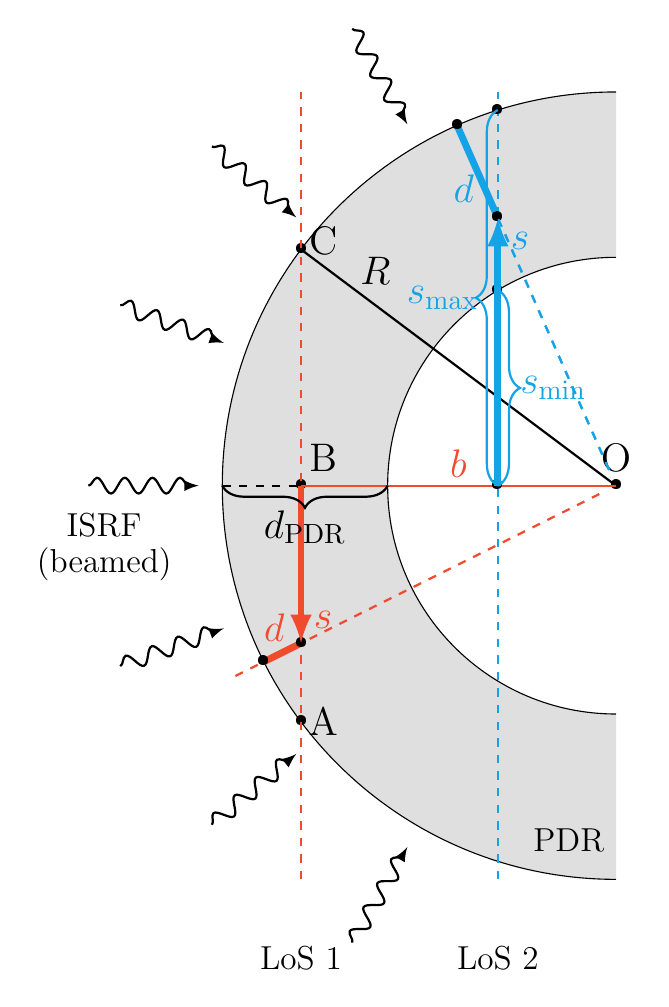
\begin{tikzpicture}
    
    \path [fill=lightgray!50]
        (0, 2.9) arc[start angle=90, end angle=270, radius=2.9] -- 
        (0, -5) arc[start angle=270, end angle=90, radius=5] -- 
        cycle;
    \draw [-, name path=outer surface] (0, 5) arc[start angle=90, end angle=270, radius=5];
    \draw [-, name path=inner surface](0, 2.9) arc[start angle=90, end angle=270, radius=2.9];
    
    \node at (-0.6, -4.5) {\large PDR};

    \node (O) at (0, 0) {\textbullet};
    \node[yshift=1em] at (0, 0) {\Large O};
    
    \node (B) at (-4, 0) {\textbullet};
    \node[yshift=1em,xshift=.8em] at (-4, 0) {\Large B};
    
    \node (A) at (-4, -3) {\textbullet};
    \node[xshift=.8em] at (-4, -3) {\Large A};

    \node (C) at (-4, 3) {\textbullet};
    \node[xshift=.8em, yshift=.3em] at (-4, 3) {\Large C};

    \node (D) at (-5, -2.5) {};
    
    \draw[thick, dashed, name path=A--C, RedOrange] (-4, -5) -- (-4, 5);
    \node at (-4, -6) {\large LoS 1};

    \draw[thick] (-4, 3) -- (0, 0) node[midway,yshift=3.5em,xshift=-3em]{\Large $R$};

    \draw[thick, dashed, name path=O--B] (-5, 0) -- (0, 0);
    
    \draw[thick, dashed, name path=O--D, RedOrange] (O) -- (D);

    \path[name intersections={of=A--C and O--D, by=P}];
    \path[name intersections={of=O--D and outer surface, by=Q}];
    \draw[line width=2.5pt, RedOrange] (P) -- (Q) node[midway,yshift=0.9em,xshift=-0.3em]{\Large $d$};
    \node at (P) {\textbullet};
    \node at (Q) {\textbullet};

    \draw[thick, RedOrange] (0, 0) -- (-4, 0) node[midway,yshift=.8em, RedOrange]{\Large $b$};
    \draw[line width=2.5pt, -latex, RedOrange] (-4, 0) -- (P) node[midway,xshift=0.8em,yshift=-2em]{\Large $s$};
    
    \draw[thick, decorate, decoration={brace,amplitude=8pt}] (-2.9, 0) -- (-5, 0) node[midway,yshift=-1.5em]{\Large $d_\mathrm{PDR}$};
    
    % second LoS
    \draw[thick, dashed, name path=A'--C', Cerulean] (-1.5, -5) -- (-1.5, 5);
    \node at (-1.5, -6) {\large LoS 2};
    \path[name intersections={of=A'--C' and outer surface, by=E}];
    \path[name intersections={of=A'--C' and inner surface, by=F}];
    \path[name intersections={of=A'--C' and O--B, by=G}];
    \node at (E) {\textbullet};
    \node at (F) {\textbullet};
    \node at (-1.5, 0) {\textbullet};
    \draw[line width=2.5pt, -latex, Cerulean] (-1.5, 0) -- (-1.5, 3.4) node[midway,xshift=0.8em,yshift=4em]{\Large $s$};
    \draw[line width=2.5pt, Cerulean] (-1.5, 3.4) -- (-2.018, 4.574) node[midway,yshift=-0.6em,xshift=-0.5em]{\Large $d$};
    \node (P') at (-1.5, 3.4) {\textbullet};
    \draw[thick, dashed, name path=O--P', Cerulean] (O) -- (P');
    % \path[name intersections={of=O--P' and outer surface, by=Q'}];
    \node (Q') at (-2.018, 4.574) {\textbullet};
    \draw[thick, dashed, Cerulean] (O) -- (Q');
    
    \draw[thick, decorate, decoration={brace,amplitude=8pt}, Cerulean] (F) -- (G) node[midway,xshift=2em]{\Large $s_\mathrm{min}$};
    \draw[thick, decorate, decoration={brace,amplitude=8pt}, Cerulean] (G) -- (E) node[midway,xshift=-2em]{\Large $s_\mathrm{max}$};

    \foreach \angle in {120, 140, 160, 180, 200, 220, 240} {
    \draw [thick, decorate, decoration={snake, amplitude=0.1cm}, -latex]
        ({6.7*cos(\angle)}, {6.7*sin(\angle)}) -- ({5.3*cos(\angle)}, {5.3*sin(\angle)});
    }
    \node at (-6.5, -0.5) {\large ISRF};
    \node at (-6.5, -1) {\large (beamed)};
        
\end{tikzpicture}

% slab geometry
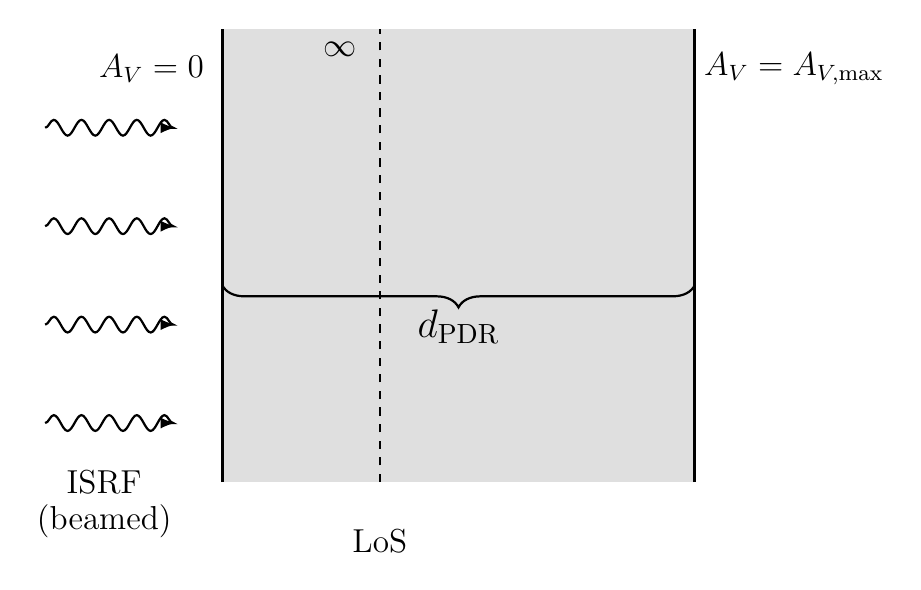
\begin{tikzpicture}
    \pgfmathsetmacro{\halfdepth}{2.5}
    \pgfmathsetmacro{\halfwidth}{3}
    
    \path [fill=lightgray!50] 
        (-\halfwidth, -\halfdepth) -- (\halfwidth, -\halfdepth) -- (\halfwidth, 1.3*\halfdepth) -- (-\halfwidth, 1.3*\halfdepth) -- cycle;
        
    \draw [very thick, -, name path=front] (-\halfwidth, -\halfdepth) -- (-\halfwidth, 1.3*\halfdepth);
    \node at (-1.3*\halfwidth, 1.1*\halfdepth) {\large $A_V = 0$};
    \draw [very thick, -, name path=back] (\halfwidth, -\halfdepth) -- (\halfwidth, 1.3*\halfdepth);
    \node at (1.42*\halfwidth, 1.1*\halfdepth) {\large $A_V = A_{V,\max}$};

    \draw [thick, decorate, decoration={brace,amplitude=8pt}] (\halfwidth, 0) -- (-\halfwidth, 0) node[midway,yshift=-1.5em]{\Large $d_\mathrm{PDR}$};

    \draw [thick, dashed] (-1, -\halfdepth) -- (-1, 1.3*\halfdepth);
    \node at (-1, -1.3*\halfdepth) {\large LoS};
    \node at (-1.5, 1.2*\halfdepth) {\large $\infty$};

    \draw [thick, decorate, decoration={snake, amplitude=0.1cm}, -latex] (-1.75*\halfwidth, 0.8*\halfdepth) -- (-1.2*\halfwidth, 0.8*\halfdepth);
    \draw [thick, decorate, decoration={snake, amplitude=0.1cm}, -latex] (-1.75*\halfwidth, 0.3*\halfdepth) -- (-1.2*\halfwidth, 0.3*\halfdepth);
    \draw [thick, decorate, decoration={snake, amplitude=0.1cm}, -latex] (-1.75*\halfwidth, -0.2*\halfdepth) -- (-1.2*\halfwidth, -0.2*\halfdepth);
    \draw [thick, decorate, decoration={snake, amplitude=0.1cm}, -latex] (-1.75*\halfwidth, -0.7*\halfdepth) -- (-1.2*\halfwidth, -0.7*\halfdepth);
    \node at (-1.5*\halfwidth, -\halfdepth) {\large ISRF};
    \node at (-1.5*\halfwidth, -1.2*\halfdepth) {\large (beamed)};
    
\end{tikzpicture}

% slab to sphere
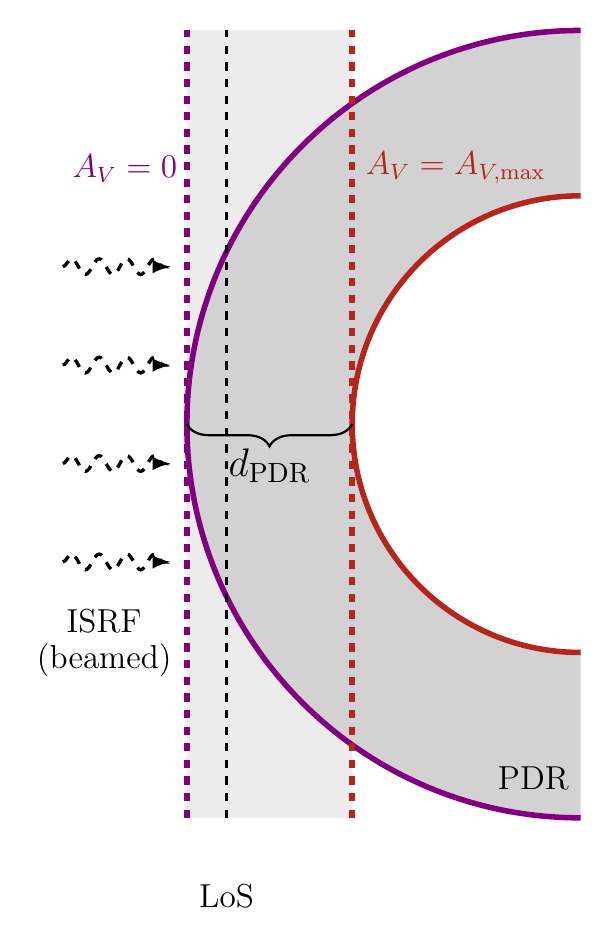
\begin{tikzpicture}
    \pgfmathsetmacro{\halfdepth}{2.5}
    \pgfmathsetmacro{\halfwidth}{1.05}
    \pgfmathsetmacro{\outerrad}{5}
    \pgfmathsetmacro{\innerrad}{2.9}
    
    \path [fill=lightgray!30] 
        (-\halfwidth, -\outerrad) -- (\halfwidth, -\outerrad) -- (\halfwidth, \outerrad) -- (-\halfwidth, \outerrad) -- cycle;
    \path [fill=lightgray!70]
        (\outerrad - \halfwidth, \innerrad) arc[start angle=90, end angle=270, radius=\innerrad] -- 
        (\outerrad - \halfwidth, -\outerrad) arc[start angle=270, end angle=90, radius=\outerrad] -- 
    cycle;
    \node at (\outerrad - \halfwidth-0.6, -4.5) {\large PDR};

    \draw [line width=2pt, -, Purple, name path=outer surface] (\outerrad - \halfwidth, \outerrad) arc[start angle=90, end angle=270, radius=\outerrad];
    \draw [line width=2pt, -, BrickRed, name path=inner surface] (\outerrad - \halfwidth, \innerrad) arc[start angle=90, end angle=270, radius=\innerrad];
        
    \draw [line width=2pt, dashed, Purple, name path=front] (-\halfwidth, -\outerrad) -- (-\halfwidth, \outerrad);
    \node at (-1.75*\halfwidth, 1.3*\halfdepth) {\textcolor{Purple}{\large $A_V = 0$}};
    \draw [line width=2pt, dashed, BrickRed, name path=back] (\halfwidth, -\outerrad) -- (\halfwidth, \outerrad);
    \node at (2.25*\halfwidth, 1.3*\halfdepth) {\textcolor{BrickRed}{\large $A_V = A_{V,\max}$}};

    \draw [thick, decorate, decoration={brace,amplitude=8pt}] (\halfwidth, 0) -- (-\halfwidth, 0) node[midway,yshift=-1.5em]{\Large $d_\mathrm{PDR}$};

    \draw [thick, dashed] (-0.52*\halfwidth, -\outerrad) -- (-0.52*\halfwidth, \outerrad);
    \node at (-0.52*\halfwidth, -\outerrad-1) {\large LoS};

    \draw [very thick, dashed, decorate, decoration={snake, amplitude=0.1cm}, -latex] (-2.5*\halfwidth, 0.8*\halfdepth) -- (-1.2*\halfwidth, 0.8*\halfdepth);
    \draw [very thick, dashed, decorate, decoration={snake, amplitude=0.1cm}, -latex] (-2.5*\halfwidth, 0.3*\halfdepth) -- (-1.2*\halfwidth, 0.3*\halfdepth);
    \draw [very thick, dashed, decorate, decoration={snake, amplitude=0.1cm}, -latex] (-2.5*\halfwidth, -0.2*\halfdepth) -- (-1.2*\halfwidth, -0.2*\halfdepth);
    \draw [very thick, dashed, decorate, decoration={snake, amplitude=0.1cm}, -latex] (-2.5*\halfwidth, -0.7*\halfdepth) -- (-1.2*\halfwidth, -0.7*\halfdepth);
    \node at (-2*\halfwidth, -\halfdepth) {\large ISRF};
    \node at (-2*\halfwidth, -1.2*\halfdepth) {\large (beamed)};
    
\end{tikzpicture}

\end{document}